\documentclass[11pt]{article}
\usepackage{tikz}
\usepackage{graphicx}
\usepackage[a4paper,margin=1in]{geometry}
\usepackage{amsmath,amssymb,amsthm}
\usepackage{mathtools}
\usepackage[T1]{fontenc}
\usepackage{lmodern}
\usepackage{microtype}

\newtheorem{theorem}{Theorem}
\newtheorem{lemma}{Lemma}
\newtheorem{definition}{Definition}
\newtheorem{remark}{Remark}

\DeclareMathOperator*{\argmin}{arg\,min}
\DeclareMathOperator*{\argmax}{arg\,max}

\newcommand{\machinerow}[2]{
    \node[machine, anchor=east] at (-0.3,-#1+0.5) {$M_{#2}$};
}

\newcommand{\dotsrow}[1]{%
    \foreach \dy in {-0.18,0,0.18} { % chktex 1
        \fill (-0.6,{-#1+0.5+\dy}) circle[radius=0.025];
        \fill (2,{-#1+0.5+\dy}) circle[radius=0.025];
    }
}

\newcommand{\jobblock}[5][white]{%
    \draw[job, fill=#1] (#3, -#2) rectangle ++ (#4,1);
    \node at ({#3 + #4/2},{-#2 + 0.5}) {$#5$}; % chktex 1
}

\newcommand{\schedulebeforeunification}{
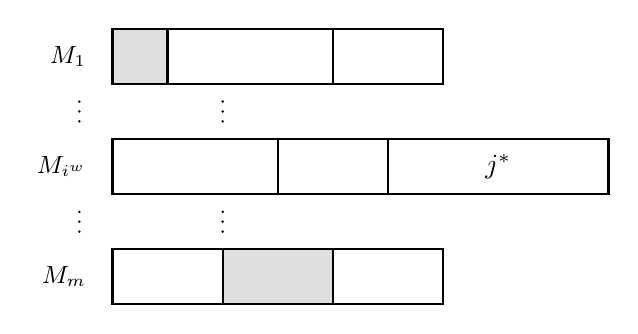
\begin{tikzpicture}[
    x=0.7cm,
    y=0.7cm,
    job/.style={
        draw,
        thick,
        fill=white,
        font=\small
    },
    machine/.style={font=\small}
]

% Displayed machine rows
\machinerow{1}{1}
\dotsrow{2}
\machinerow{3}{i^{w}}
\dotsrow{4}
\machinerow{5}{m}

% Edit the first schedule here.
\jobblock[gray!25]{1}{0}{1}{}
\jobblock{1}{1}{3}{}
\jobblock{1}{4}{2}{}


\jobblock{3}{0}{3}{}
\jobblock{3}{3}{2}{}
\jobblock{3}{5}{4}{j^{*}}

\jobblock{5}{0}{2}{}
\jobblock[gray!25]{5}{2}{2}{}
\jobblock{5}{4}{2}{}

\end{tikzpicture}
}

\newcommand{\scheduleafterunification}{
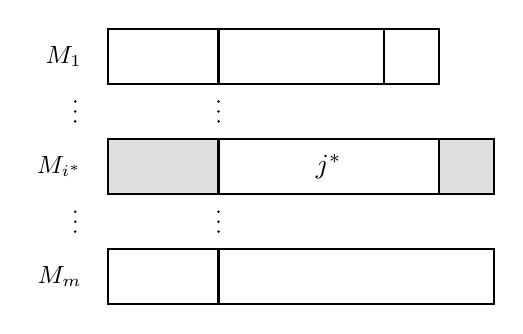
\begin{tikzpicture}[
    x=0.7cm,
    y=0.7cm,
    job/.style={
        draw,
        thick,
        fill=white,
        font=\small
    },
    machine/.style={font=\small}
]

% Displayed machine rows
\machinerow{1}{1}
\dotsrow{2}
\machinerow{3}{i^{*}}
\dotsrow{4}
\machinerow{5}{m}

% Edit the second schedule here.
\jobblock{1}{0}{2}{}
\jobblock{1}{2}{3}{}
\jobblock{1}{5}{1}{}

\jobblock[gray!25]{3}{0}{2}{}
\jobblock{3}{2}{4}{j^{*}}
\jobblock[gray!25]{3}{6}{1}{}

\jobblock{5}{0}{2}{}
\jobblock{5}{2}{5}{}


\end{tikzpicture}
}

\newcommand{\scheduleclosetimegaps}{
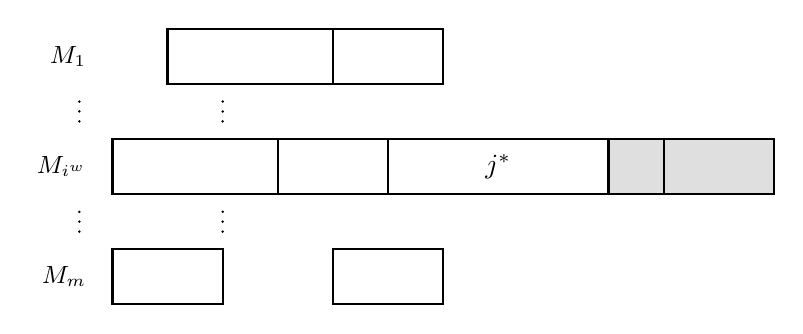
\begin{tikzpicture}[
    x=0.7cm,
    y=0.7cm,
    job/.style={
        draw,
        thick,
        fill=white,
        font=\small
    },
    machine/.style={font=\small}
]
% Displayed machine rows
\machinerow{1}{1}
\dotsrow{2}
\machinerow{3}{i^{w}}
\dotsrow{4}
\machinerow{5}{m}

% Edit the third schedule here.

\jobblock{1}{1}{3}{}
\jobblock{1}{4}{2}{}


\jobblock{3}{0}{3}{}
\jobblock{3}{3}{2}{}
\jobblock{3}{5}{4}{j^{*}}
\jobblock[gray!25]{3}{9}{1}{}
\jobblock[gray!25]{3}{10}{2}{}

\jobblock{5}{0}{2}{}

\jobblock{5}{4}{2}{}

\end{tikzpicture}
}

\newcommand{\schedulereschedulelastjobs}{
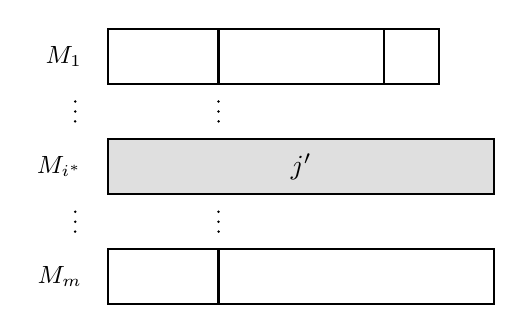
\begin{tikzpicture}[
    x=0.7cm,
    y=0.7cm,
    job/.style={
        draw,
        thick,
        fill=white,
        font=\small
    },
    machine/.style={font=\small}
]

% Displayed machine rows
\machinerow{1}{1}
\dotsrow{2}
\machinerow{3}{i^{*}}
\dotsrow{4}
\machinerow{5}{m}

% Edit the fourth schedule here.
\jobblock{1}{0}{2}{}
\jobblock{1}{2}{3}{}
\jobblock{1}{5}{1}{}


\jobblock[gray!25]{3}{0}{7}{j'}


\jobblock{5}{0}{2}{}
\jobblock{5}{2}{5}{}

\end{tikzpicture}
}

\newcommand{\schedulelistschedule}{
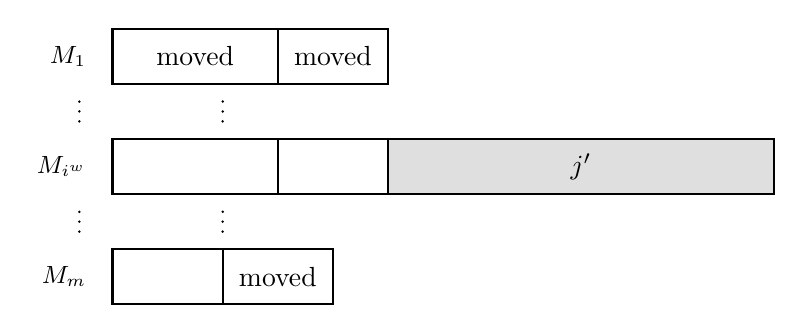
\begin{tikzpicture}[
    x=0.7cm,
    y=0.7cm,
    job/.style={
        draw,
        thick,
        fill=white,
        font=\small
    },
    machine/.style={font=\small}
]

% Displayed machine rows
\machinerow{1}{1}
\dotsrow{2}
\machinerow{3}{i^{w}}
\dotsrow{4}
\machinerow{5}{m}

% Edit the fifth schedule here.
\jobblock{1}{0}{3}{\text{moved}}
\jobblock{1}{3}{2}{\text{moved}}


\jobblock{3}{0}{3}{}
\jobblock{3}{3}{2}{}
\jobblock[gray!25]{3}{5}{7}{j'}


\jobblock{5}{0}{2}{}
\jobblock{5}{2}{2}{\text{moved}}

\end{tikzpicture}
}

\newcommand{\schedulefinalworst}{
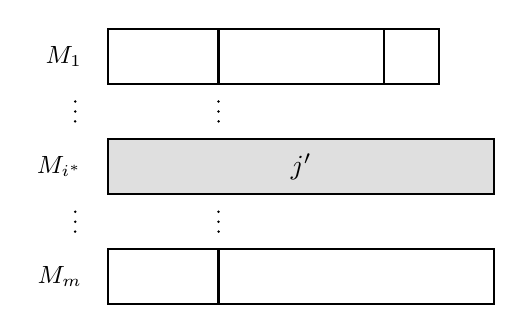
\begin{tikzpicture}[
    x=0.7cm,
    y=0.7cm,
    job/.style={
        draw,
        thick,
        fill=white,
        font=\small
    },
    machine/.style={font=\small}
]

\machinerow{1}{1}
\dotsrow{2}
\machinerow{3}{i^{*}}
\dotsrow{4}
\machinerow{5}{m}

% Edit the sixth schedule here.
\jobblock{1}{0}{2}{}
\jobblock{1}{2}{3}{}
\jobblock{1}{5}{1}{}


\jobblock[gray!25]{3}{0}{7}{j'}


\jobblock{5}{0}{2}{}
\jobblock{5}{2}{5}{}

\end{tikzpicture}
}

\newcommand{\scheduleseventh}{
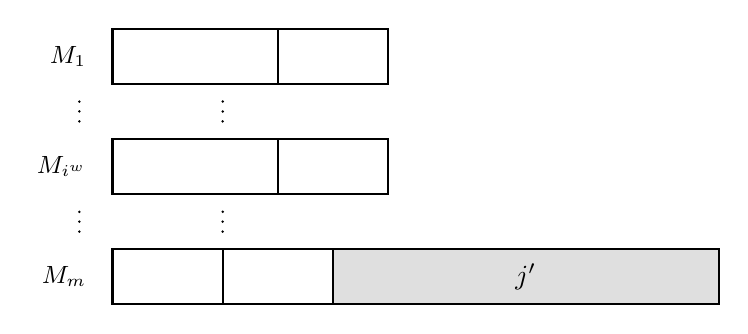
\begin{tikzpicture}[
    x=0.7cm,
    y=0.7cm,
    job/.style={
        draw,
        thick,
        fill=white,
        font=\small
    },
    machine/.style={font=\small}
]

\machinerow{1}{1}
\dotsrow{2}
\machinerow{3}{i^{w}}
\dotsrow{4}
\machinerow{5}{m}

% Edit the seventh schedule here.
\jobblock{1}{0}{3}{}
\jobblock{1}{3}{2}{}


\jobblock{3}{0}{3}{}
\jobblock{3}{3}{2}{}



\jobblock{5}{0}{2}{}
\jobblock{5}{2}{2}{}
\jobblock[gray!25]{5}{4}{7}{j'}
\end{tikzpicture}
}

\newcommand{\scheduleeighth}{
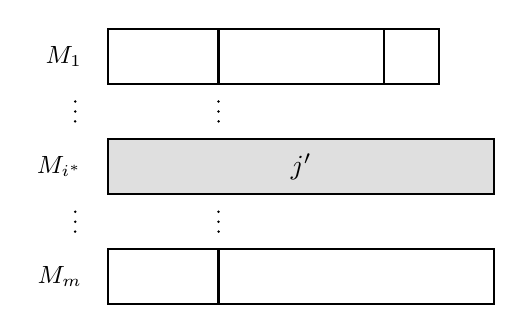
\begin{tikzpicture}[
    x=0.7cm,
    y=0.7cm,
    job/.style={
        draw,
        thick,
        fill=white,
        font=\small
    },
    machine/.style={font=\small}
]

\machinerow{1}{1}
\dotsrow{2}
\machinerow{3}{i^{*}}
\dotsrow{4}
\machinerow{5}{m}

% Edit the eighth schedule here.
\jobblock{1}{0}{2}{}
\jobblock{1}{2}{3}{}
\jobblock{1}{5}{1}{}

\jobblock[gray!25]{3}{0}{7}{j'}

\jobblock{5}{0}{2}{}
\jobblock{5}{2}{5}{}

\end{tikzpicture}
}

\begin{document}

\title{Single-Machine Schedule Lemma}
\author{}
\date{}
\maketitle

\section{Statement}

\begin{definition}[Single scheduled job]
Let \(I\) be an instance of the \(P||\sum_{j=1}^{n}{p_j C_j}(\alpha)\) scheduling problem.
We call a job $single scheduled$ in a schedule $S$ if it is the only job scheduled on its machine in $S$.
\end{definition}

\begin{lemma} \label{lemma: Peak increase }
Let $x_1,\dots,x_n \in \mathbb{R}$ satisfy
\[
\sum_{i=1}^n x_i = c,
\]
and suppose that $x_1 \ge x_i$ for all $i=2,\dots,n$. Let $\delta\geq0$, and let
$\delta_2,\dots,\delta_n \ge 0$ satisfy
\[
\sum_{i=2}^n \delta_i = \delta.
\]
Define
\[
x_1' = x_1+\delta,
\qquad
x_i' = x_i-\delta_i \quad \text{for } i=2,\dots,n.
\]
Then
\[
\sum_{i=1}^n (x_i')^2 \geq \sum_{i=1}^n x_i^2.
\]
If \(\delta>0\), then the inequality is strict.
\end{lemma}

\begin{proof}
We compute
\[
\sum_{i=1}^n (x_i')^2-\sum_{i=1}^n x_i^2
=
(x_1+\delta)^2-x_1^2
+
\sum_{i=2}^n \left((x_i-\delta_i)^2-x_i^2\right).
\]
Expanding gives
\[
2\delta x_1+\delta^2
-
2\sum_{i=2}^n \delta_i x_i
+
\sum_{i=2}^n \delta_i^2.
\]
Using $\delta=\sum_{i=2}^n \delta_i$, this equals
\[
2\sum_{i=2}^n \delta_i(x_1-x_i)
+
\delta^2
+
\sum_{i=2}^n \delta_i^2.
\]
Since $x_1\ge x_i$ and $\delta_i\ge 0$ for all $i=2,\dots,n$, every
term in the last expression is nonnegative. Hence
\[
\sum_{i=1}^n (x_i')^2-\sum_{i=1}^n x_i^2 \geq 0.
\]
If \(\delta>0\), then \(\delta^2>0\), so the inequality is strict.
\end{proof}

\begin{lemma}\label{lem: A,B,C,r}
Let
\[
A>C>B\ge 0,\qquad r\geq0,\qquad d>0,\qquad B+d<C
\qquad \text{and} \qquad \alpha \in [0, \frac12].
\]
Then: 
\[
\frac{A+(2\alpha-1)B}{C+(2\alpha-1)B}
\le
\frac{A+r+(2\alpha-1)(B+d)}{C+(2\alpha-1)(B+d)}.
\]
If \(\alpha<\frac12\), then the inequality is strict.
\end{lemma}

\begin{proof}
    
Let
\[
x=1-2\alpha.
\]
Since \(\alpha\in[0,\frac12]\), we have \(x\in[0,1]\). The inequality becomes
\[
\frac{A-xB}{C-xB}
\le
\frac{A+r-x(B+d)}{C-x(B+d)}.
\]

Both denominators are positive. Equivalently:
\[
(A-xB)\bigl(C-x(B+d)\bigr)
\le
\bigl(A+r-x(B+d)\bigr)(C-xB).
\]
After cancellation, this is equivalent to
\[
r(C-xB)+x(A-C)d\ge 0.
\]

Since \(x\in[0,1]\) and \(C>B\geq0\), we have \(C-xB>0\).
Moreover, \(r\geq0\), \(x\geq0\), \(A-C>0\), and \(d>0\).
Thus both terms in the last expression are nonnegative, which proves the
inequality.
If \(\alpha<\frac12\), then \(x>0\), so
\(x(A-C)d>0\). Hence the inequality is strict in this case.
\end{proof}

\begin{lemma}[Single scheduled]
Let $I$ be an instance of the $P||\sum_{j=1}^{n}{p_j C_j}(\alpha)$ scheduling problem.
If $\alpha \leq \frac{1}{2}$, then there exists an instance $I'$ of the $P||\sum_{j=1}^{n}{p_j C_j}(\alpha)$ 
scheduling problem $j'$, for which there exists an optimal schedule $S_{OPT}(I')$ with
at least one single scheduled job such that: 
\begin{align*}
   \lambda(I)(\alpha) \geq \lambda(I')(\alpha) 
\end{align*} 
Furthermore, there exists a worst schedule $S_{W}(I')$, in which no job finishes after $j'$. 
\end{lemma}

\begin{proof}
We prove the claim by constructing an instance with the single schedule property from any instance of $P||\sum_{j=1}^{n}{p_j C_j}(\alpha)$ with larger or equal $\lambda$ value.
We assume the initial step of reduction through unification was performed on $I$.

Consider any $I$ of $P||\sum_{j=1}^{n}{p_j C_j}(\alpha)$, and fix any pair $S_{WORST},S_{OPT}$. Fix $j^*$ to be any job that finishes last in $S_{WORST}$.
Let $i^*$ be the machine on which $j^*$ is scheduled in $S_{OPT}$. 
Unify (according to reference here to unifying def.) all jobs scheduled on $i^*$ in $S_{OPT}$ to a single job $j'$. 
The first observation is that: 
\[
C^{i}_{\max}(S_{OPT}(I)) = C^{i}_{\max}(S_{OPT}(I')) \quad \forall i \in [m].
\]
where $I'$ is the instance that differs from $I$ only through unification to $j'$.

Next we consider what happens to the schedule $S_{WORST}$ when we unify the jobs on $i^*$ to $j'$.
To this end, let $i^{w}$ be the machine on which $j^*$ is scheduled in $S_{WORST}$ in instance $I$.

Beginning with $S_{WORST}$ we perform the following construction steps: 

\begin{enumerate}
    \item Move all jobs that were affected by unification except $j^*$, to be scheduled after $j^*$ on $i^{w}$.
     This can now be considered as the unified job $j'$.
    \item Close any idle time gaps in the schedule by canonically moving jobs back.
    \item Reschedule the subset of jobs that are last scheduled on a machine but are not scheduled according to list scheduling.
    \item The resulting schedule is named $S'_{WORST}$.
\end{enumerate}
\begin{figure}[p]
\centering
\setlength{\fboxsep}{6pt}
\fbox{%
\begin{minipage}{0.94\textwidth}
    \begin{minipage}[t]{0.47\linewidth}
        \centering
        \resizebox{\linewidth}{!}{\schedulebeforeunification}
        \par\smallskip
        \small(a) \(S_{WORST}(I)\)
    \end{minipage}
    \hfill
    \begin{minipage}[t]{0.47\linewidth}
        \centering
        \resizebox{\linewidth}{!}{\scheduleafterunification}
        \par\smallskip
        \small(b) \(S_{OPT}(I)\)
    \end{minipage}
    \par\smallskip
    \centering\small Initial schedules of $I$.
\end{minipage}%
}

\medskip

\fbox{%
\begin{minipage}{0.94\textwidth}
    \begin{minipage}[t]{0.47\linewidth}
        \centering
        \resizebox{\linewidth}{!}{\scheduleclosetimegaps}
        \par\smallskip
        \small(c) Moving jobs from $M_{i^*}$ to $M_{i^{w}}$
    \end{minipage}
    \hfill
    \begin{minipage}[t]{0.47\linewidth}
        \centering
        \resizebox{\linewidth}{!}{\schedulereschedulelastjobs}
        \par\smallskip
        \small(d) Unification
    \end{minipage}
    \par\smallskip
    \centering\small  1.
\end{minipage}%
}

\medskip

\fbox{%
\begin{minipage}{0.94\textwidth}
    \begin{minipage}[t]{0.47\linewidth}
        \centering
        \resizebox{\linewidth}{!}{\schedulelistschedule}
        \par\smallskip
        \small(e) Removing idle time
    \end{minipage}
    \hfill
    \begin{minipage}[t]{0.47\linewidth}
        \centering
        \resizebox{\linewidth}{!}{\schedulefinalworst}
        \par\smallskip
        \small(f) \(S'_{OPT}(I')\)
    \end{minipage}
    \par\smallskip
    \centering\small 2.
\end{minipage}%
}

\medskip

\fbox{%
\begin{minipage}{0.94\textwidth}
    \begin{minipage}[t]{0.47\linewidth}
        \centering
        \resizebox{\linewidth}{!}{\scheduleseventh}
        \par\smallskip
        \small(g) \(S'_{WORST}(I')\)
    \end{minipage}
    \hfill
    \begin{minipage}[t]{0.47\linewidth}
        \centering
        \resizebox{\linewidth}{!}{\scheduleeighth}
        \par\smallskip
        \small(h) \(S'_{OPT}(I')\)
    \end{minipage}
    \par\smallskip
    \centering\small 3.
\end{minipage}%
}
\caption{Schedule construction}\label{fig:schedule-structure}
\end{figure}

The following properties remain to be shown: 
\begin{itemize}
    \item $S'_{WORST}$ is a list schedule of $I'$.
    \item $S'_{OPT}$ is a list schedule of $I'$.
    \item $\lambda(I')(\alpha) \geq \lambda(I)(\alpha) \quad \forall \alpha \leq \frac{1}{2}$.
\end{itemize}

It is easy to see that $S'_{OPT}$ is a list schedule of $I'$. 
As if this is not the case, then $S_{OPT}$ is not a list schedule of $I$, which is a contradiction to 
its optimality. 

Similarly, $S'_{WORST}$ is a list schedule of $I'$, as in step 3, we reschedule all jobs that might not be scheduled
according to a list. It is therefore true by construction. 



Finally, we show that 
\[
    \lambda(I')(\alpha) \geq \lambda(I)(\alpha) \quad \forall \alpha \leq \frac{1}{2}.
\]

To this end, we can say that each machine only contributes one job to unification
in $S_{WORST}$. This is because, else we could have performed a step of unification according to
(again original unification reference here).
Next, we reason for:  
\[
C_{max}^{max}(S'_{WORST}(I')) \geq C_{max}^{max}(S_{WORST}(I))
\]

We consider two cases. 
\begin{enumerate}
    \item   $j^*$ is not rescheduled. As $j^*$ was the last job to complete in $S_{WORST}(I)$ and we do not 
            increase the processing time for any other machine than $i_{w}$, this still is the case for $S'_{WORST}(I')$. 
            If $p_{j'} = p_{j^*}$ then this implies that $p_{j^*}$ was already a single scheduled job in $S_{OPT}(I)$. 
            The only other case is: $p_{j'}  > p_{j^*}$. Since the start time of both jobs is equal in their respective worst 
            schedules, this implies: 
            \begin{align*}
            C_{max}^{max}(S'_{WORST}(I'))>C_{max}^{max}(S_{WORST}(I)).
            \end{align*}
    \item  Assume without loss of generality, that $j^{*}$ is rescheduled to machine $m$ in the construction process.
            (as depicted in (e) to (g)). Since $j^{*}$  was not scheduled on $m$ in $S_{WORST}(I)$ it must hold, that the starting time 
            of $j^*$ is smaller or equal to $C^{m}_{max}(S_{WORST}(I))$. The rescheduling of $j^{*}$ to $m$ implies that a job
            that was scheduled on $m$ in $S_{WORST}(I)$ was unified with $j^*$ to $j'$. This means, that the new load on machine $m$ is now at least as
            large as the load on machine $i_{w}$ in $S_{WORST}(I)$. So: 
            \begin{align*}
            C_{max}^{max}(S'_{WORST}(I')) \ge C_{max}^{max}(S_{WORST}(I))
            \end{align*}
\end{enumerate}


Now since $\sum_{j=1}^{n}p_j$ is fixed, $\sum_{i=1}^{m}C^{max}_i(\sigma(I))$ is also fixed for any instance, we can apply \ref{lemma: Peak increase }

with \[x_1 = C^{max}_{max}(S_{WORST}(I)) \qquad x'_1 = C^{max}_{max}(S'_{WORST}(I'))\]

and 

\[
x_i = C^{max}_i(S_{WORST}(I)) \forall i [2,\dots, m] \qquad \delta_i = p_{j(i)}
\]
where $j(i)$ is the job on machine i in $S_{WORST}$ that gets unified with $j^*$ in (2).
If such a job does not exist for some $i$, set $p_{j(i)} = 0$ 

We can apply \ref{lemma: Peak increase } to get 

\[
r:= \sum_{i=1}^m (C_i^{max}(S'_{WORST}(I')))^2 - \sum_{i=1}^m (C_i^{max}(S_{WORST}(I)))^2 \ge 0
\]

and with 
\[
A:= \sum_{i=1}^m (C_i^{max}(S_{WORST}(I)))^2 \qquad B:=\sum_{i=1}^{n}p_i^2 \qquad C:=\sum_{i=1}^m (C_i^{max}(S_{OPT}(I)))^2
\]

\[
d:= 2p_{j^*}\sum_{i\in U}p_{i}
\]

where U is the set of jobs that get unified with $j^*$. 

A final application of \ref{lem: A,B,C,r} gives the stated result.
\end{proof}

\end{document}
